\section{Methodology}
\label{sec_methodology}

In this section, we present the experimental methodology that should be used to measure the sensitivity of electronic devices to thermal and high energy neutrons. We describe the available neutron sources as well as the computing devices selected and the codes executed.

\subsection{Devices}
\label{subsec_devices}

To evaluate the sensitivity of thermal and high energy neutrons it is fundamental to test various COTS devices. The devices selected should be used in all the different domains described in Section~\ref{sec_mot}. For the co-processor, explicitly manufactured for HPC and data centers, we tested an \textbf{Intel Xeon Phi}, built using a $22nm$ Intel's 3-D Tri-gate technology. We also tested two \textbf{NVIDIA GPUs} that are used in all domains: NVIDIA K20 manufactured in a $28nm$ TSMC CMOS technology, NVIDIA TitanX fabricated in a $16nm$ TSMC FinFET technology. An \textbf{AMD Accelerated Processing Unit (APU)}, manufactured in a $28nm$ SHP Bulk Process at Global Foundries is a hybrid device that can also be used in all domains. The APU integrates CPU and GPU in the same chip. Finally, Zynq-7000 is the \textbf{FPGA} tested, fabricated in a $28nm$ TSMC technology.

\subsection{Codes}
\label{subsec_codes}

The code selection needs to consider the devices in which they are going to be executed. They have a wide range of architectural and computational characteristics. Then, to have a fair evaluation, we selected codes that are efficient for each device, so we can reduce the bias in the reliability evaluation toward devices that are more efficient for the codes.

A matrix multiplication, LUD, LavaMD, and HotSpot were selected for Xeon Phi and GPUs. These codes are highly arithmetic codes that solve linear algebra and finite difference methods, which are executed efficiently in HPC devices. For APU, which is a heterogeneous device, we use SC, CED, and BFS that are made specifically for such devices. Finally, we also tested YOLO and MNIST to represent neural networks. These neural networks were tested in GPUs and FPGAs to evaluate the impact on self-driven vehicles.

\subsection{Radiation Experiments Setup}
\label{sub_beam_setup}

The amount of $^{10}B$ involved in the manufacturing process is part of the industry sensitive data and is definitely not publicly available. Actually, the quantity of Boron can even vary from a batch of devices to another. That said, a customer can ask (paying) to the fab to reduce the amount of Boron or to use high quality products to significantly reduced the amount of $^{10}B$. When evaluating the reliability of COTS devices for applications in which reliability matters, thermal neutrons should be considered. Radiation experiments are the only way to evaluate if the device meets the project reliability requirements considering also thermal neutrons. To achieve this evaluation it is necessary to expose the device to both high energy and thermal neutrons, comparing the sensitivity of the device to both kind of neutrons.

There are some facilities that allow to measure the realistic error rates of computing devices to high energy neutrons, such as the Los Alamos National Lab's Los Alamos Neutron Science Center in the US or the ChipIR facility of the Rutherford Appleton Lab in the UK. Thermal neutrons are used for physics of matter studies and there are not dedicated beam line for the test of electronic devices. However, as shown in~\ref{jsc2020}, it is possible to adapt thermal neutrons facilities for the test of computing systems. Reactors, such as the ones available in nuclear power plants, are also excellent controlled sources for thermal neutrons.

\subsection{Thermal Neutrons Detector}
\label{sub_detector}

We deployed Tin-II, which is a thermal neutron detector,  to measure the actual thermal neutrons flux in certain conditions. Tin-II will be used to evaluate the thermal neutrons flux inside the Trinity supercomputer at LANL.  We used Tin-II to evaluate the effect of surrounding materials in modern data centers on thermal neutrons flux. We evaluated the impact of liquid cooling by counting thermal neutrons with and without a box containing 2 inches of water close to the detector. The count difference, shown in detail in Section~\ref{sub_flux}, indicates the water influence in the thermal neutrons flux.

%In this section, we describe the devices and applications chosen to test the impact of high energy and thermal neutrons in modern computing devices reliability. We also detail the radiation experiments setup used for this work and describe the detector we used to measure the impact of materials in the thermal neutron flux.
%
%\subsection{Devices}
%\label{subsec_devices}
%
%We selected six devices for this study using different technologies and vendors to have an in-depth insight of thermal neutrons sensitivity on a breadth of modern devices. It is worth noting that both the fabrication process and the foundry can significantly impact the amount of $^{10}B$ in the device.
%
%\textbf{Intel Xeon Phi} is designed for HPC systems, built using a \textbf{$22nm$ Intel's 3-D Tri-gate technology}.
%
%\textbf{NVIDIA K20} is a GPU built with the $Kepler$ architecture and fabricated in a \textbf{$28nm$ TSMC CMOS technology}.
%
%\textbf{NVIDIA TitanX} is a GPU built with the $Pascal$ architecture and fabricated in a \textbf{$16nm$ TSMC FinFET technology}.
%
%\textbf{NVIDIA TitanV} is built with the $Volta$ architecture and fabricated in a \textbf{$12nm$ TSMC FinFET technology}.
%
%\textbf{AMD Accelerated Processing Unit (APU)} integrates CPU and GPU in the same chip fabricated in a \textbf{$28nm$ SHP Bulk Process at Global Foundries}.
%
%\textbf{FPGA} is the Zynq-7000 designed by Xilinx using a \textbf{$28nm$ TSMC technology}.
%
%
%\subsection{Codes}
%\label{subsec_codes}
%
%The set of devices we consider covers a wide range of architectural and computational characteristics. Using the same code for each device would bias the reliability evaluation, in favor of the devices that are more efficient in executing the chosen code. 
%To have a fair evaluation, then, we choose for each class of devices the codes that better fit with its computational characteristics. For Xeon Phi and GPUs we chose four codes representative of \textbf{HPC}: MxM, LUD, LavaMD, and HotSpot. We selected three \textbf{heterogeneous} codes specially made to fully utilize the APU architecture: SC, CED, and BFS. Finally, on GPUs and FPGA we tested two \textbf{neural networks} to represent codes that  have a significant impact on self-driven vehicles: YOLO and MNIST. 
%
%\textbf{Matrix Multiplication (MxM)} is representative of highly arithmetic compute-bound codes used in HPC and for features extraction in CNNs~\cite{Dongarra2013}. 
%
%\textbf{LUD} is a linear algebra method that calculates solutions for a square system of linear equations.
%
%\textbf{LavaMD} simulates particle interactions using Finite Difference Methods~\cite{lava2009}. 
%
%\textbf{Hotspot} is representative of stencil solvers~\cite{lava2009}, it estimates the processor temperature using an architectural
%floor plan and simulated power measurements. 
%
%\textbf{Stream Compaction (SC)} is a memory-bound code used in databases and image processing applications. SC is composed of a data manipulation primitive that removes elements from an array.
%
%\textbf{Canny Edge Detection (CED)} extracts information from images and reduce the amount of data to be processed. CPU and GPU concurrently work on different frames. 
%
%\textbf{Breadth First Search (BFS)} is a search in graphs algorithms that performs non-uniform memory access widely used in GPS Navigation Systems. 
%
%\textbf{YOLO} is a Convolution Neural Network (CNN) used for object classification and detection~\cite{yolo2015}. 
%
%\textbf{MNIST} is a CNN used for classifying handwritten digits~\cite{deng2012}. We have tested MNIST only on FPGAs as it is a minimal network that would not exercise sufficient resources on GPUs or Xeon Phis.
%
%
%\subsection{Radiation Experiments Setup}
%\label{sub_beam_setup}
%
%\begin{figure}[tb]
%\centering
%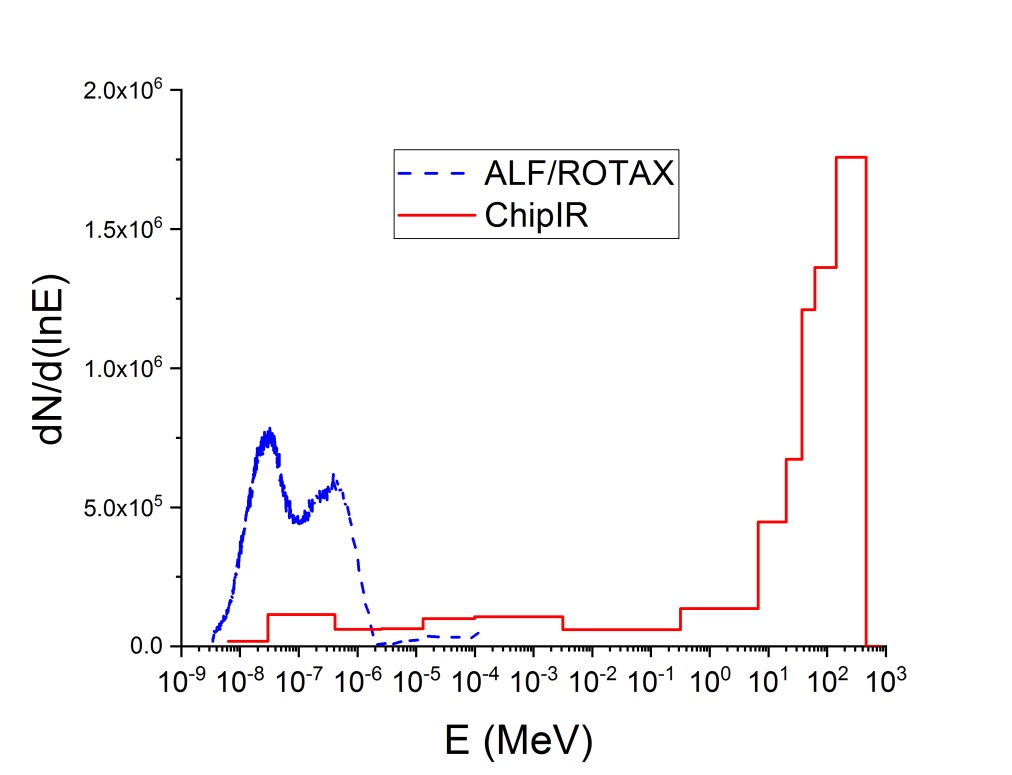
\includegraphics[width=0.35\textwidth]{./figs/rotax-chipir}
%\caption{The neutron spectra of the beamlines used for irradiation in lethargy scale.}
%\label{rotax_chipir}
%\end{figure}
%
%To evaluate the sensitivity of our devices to high energy and thermal neutrons we exposed the devices on two different beamlines at the ISIS spallation neutron source in the UK: ChipIR for high energy neutrons and ROTAX for thermal neutrons.
%ChipIR~\cite{cazzaniga2018progress} is the reference beamline dedicated to the irradiation of microelectronics and it features a high energy neutron spectrum, as similar as possible to the atmospheric one. The flux with neutron energy above 10 MeV is $5.4 \times {10}^6 n/{cm}^2/s$, while the thermal component ($E < 0.5 eV$) is $4 \times {10}^5 n/{cm}^2/s$~\cite{chiesa2018measurement}.
%ROTAX~\cite{tietze1989rotax} is a general purpose beamline with a thermal neutron spectrum generating a flux of $2.72\times{10}^6 n/{cm}^2/s$. Here the thermalization is achieved by moderation of the neutrons using liquid methane. 
%
%The spectra of the two beamlines are compared in Figure~\ref{rotax_chipir} on a log-log scale where the fluxes are proportional to the areas under the curves. As Figure~\ref{rotax_chipir} suggests, most neutrons in ROTAX are thermals and most neutron in ChipIR are high energy one.
%
%
%To evaluate the sensitivity to thermal and high energy neutrons we align the devices with the beam, while executing the codes. The device output is compared with a pre-computed fault-free copy and any mismatch is marked as an SDC. If the device stops responding we count a DUE.  To eliminate any setup-dependent differences between thermal and high energy neutrons, we irradiate the same physical devices executing the codes with the same input both in ROTAX and in ChipIR. The only difference between the two experiments is that at ChipIR we can align various boards with the beam, as shown in Figure~\ref{rad_setup}. Using a derating factor that takes distance into account we can measure the sensitivity of multiple devices in parallel. In ROTAX, as the irradiate device block most of the incoming neutrons, we must test one device at a time.
%
%
%\begin{figure}[tb]
%\centering
%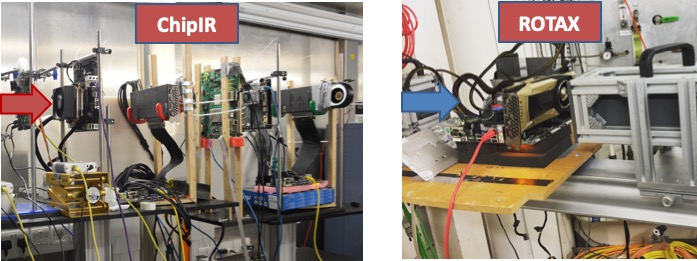
\includegraphics[width=0.80\columnwidth]{./figs/setup}
%\caption{Experimental setup in ChipIR and ROTAX. The arrow indicates the direction of the neutron beam.}
%\label{rad_setup}
%\end{figure}
%
%
%\subsection{Thermal Neutrons Detector}
%\label{sub_detector}
%
%
%We have designed and deployed a thermal neutron detector, called Tin-II, to measure the flux of thermal neutrons in different conditions. Ultimately, Tin-II will be used to measure the flux of thermal neutrons inside the data center housing the Trinity supercomputer at LANL. 
%
%Tin-II counted thermal neutron events over the course of several days. To estimate the effect of some of the characteristic materials in modern data centers on the thermal neutron flux, we placed a box containing 2 inches of water close to the detector. The count difference with and without the water, shown in details in Section~\ref{sub_flux}, indicates its influence in the thermal neutrons flux.


